\chapter{Automata models}
\label{chap:automata_models}

Here a set of automata models for some industrial entities is given. The
models are given both with no failure and failure behaviour. Failures are
reflected as events according to the event-based failure modeling approach and
as marked states for the state-based failure modeling approach. In the both
cases a marked state in a figure means that a fault occurred.  

\section{Digital Inputs/Outputs, Sensors, Motors, etc., and their connection}

\begin{figure}[th]
	\centering
	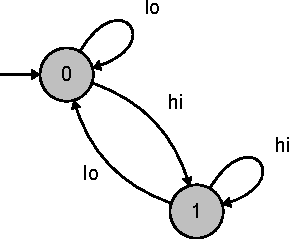
\includegraphics[scale=0.7]{lib_dido.pdf}
	\caption{General model of a digital input/output, relay, contactor, etc.}
	\label{fig:lib_dido}
\end{figure}


\begin{figure}[th]
	\centering
	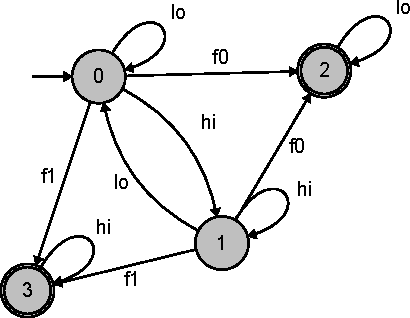
\includegraphics[scale=0.7]{lib_dido_fail.pdf}
	\caption{Model of a digital input/output with failures}
	\label{fig:lib_dido_fail}
\end{figure}

The Figure \ref{fig:lib_dido} depicts a general model of a two-state component.
This model reflects behaviour of digital inputs/outputs, relays, contactors,
motors and other devices the behaviour of which can be equal to this
abstraction. The Figure \ref{fig:lib_dido_fail} depicts a faulty version of the
model. The faulty model reflects two failures: ``stuck low'' denoted as $f0$ and
``stuck high'' denoted as $f1$.

A consequent connection of two modules as the ones described above in a
cause-effect manner imposes constrain on the ``effect'' module. Assume that
there is two modules: $1$ -- ``cause'' (e.g. a contactor) and $2$ -- ``effect''
(e.g a motor). The model of the constrain and the result of composition of the
entire system (two components and their constrain) is depicted in Figure
\ref{fig:lib_2do}. If the module $1$ has failures modeled as shown in Figure
\ref{fig:lib_dido_fail}, then the entire system looks as in Figure
\ref{fig:lib_2do_fail}.

A model of the same failure can be presented using the state-based
failure approach. In this case no fault events are used. Since the model of
a digital signal defines its full language, the model of the constrain has to be
exploited instead, as shown in the Figure \ref{fig:lib_2do_fail2}. The resulting
composition has lower complexity. It has a positive effect for the
computation burden during verification of complex systems, since almost any
industrial system includes many digital inputs, outputs and other similar
components. However, it is arguable what model should include the failure of the
component, the model of the component itself or models of constrains.


\begin{figure}[!th]
	\centering
	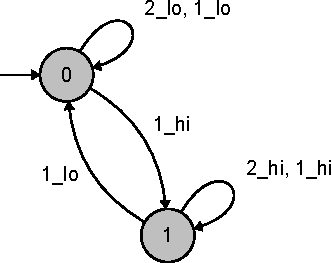
\includegraphics[scale=0.7]{lib_do2do.pdf}
	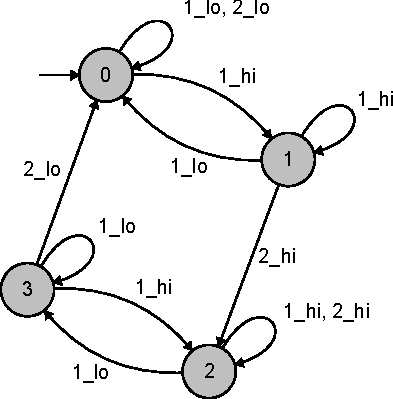
\includegraphics[scale=0.7]{lib_2do.pdf}
	\caption{The constrain model (left) for two consequent two-state components,
	and the result of the composition of the entire system (right)}
	\label{fig:lib_2do}
\end{figure}

\begin{figure}[!th]
	\centering
	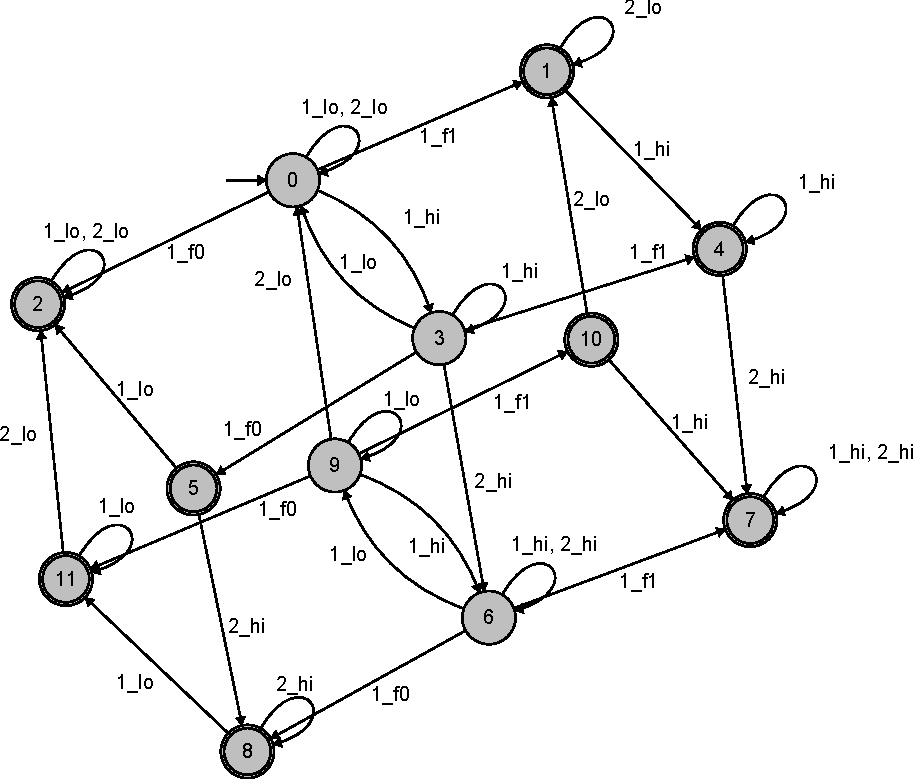
\includegraphics[scale=0.7]{lib_2do_fail.pdf}
	\caption{Fault model of two consequent digital two-state modules. The
	first module has failures}
	\label{fig:lib_2do_fail}
\end{figure}


\begin{figure}[!th]
	\centering
	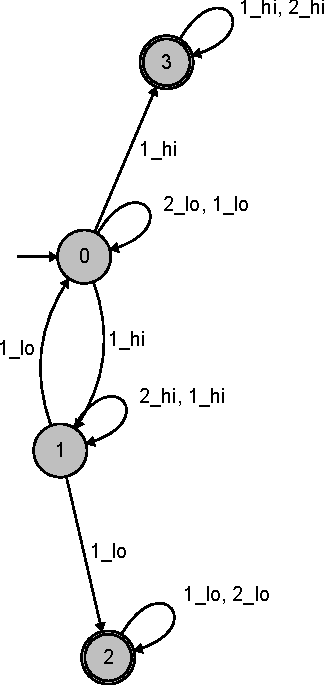
\includegraphics[scale=0.7]{lib_do2do_fail.pdf}
	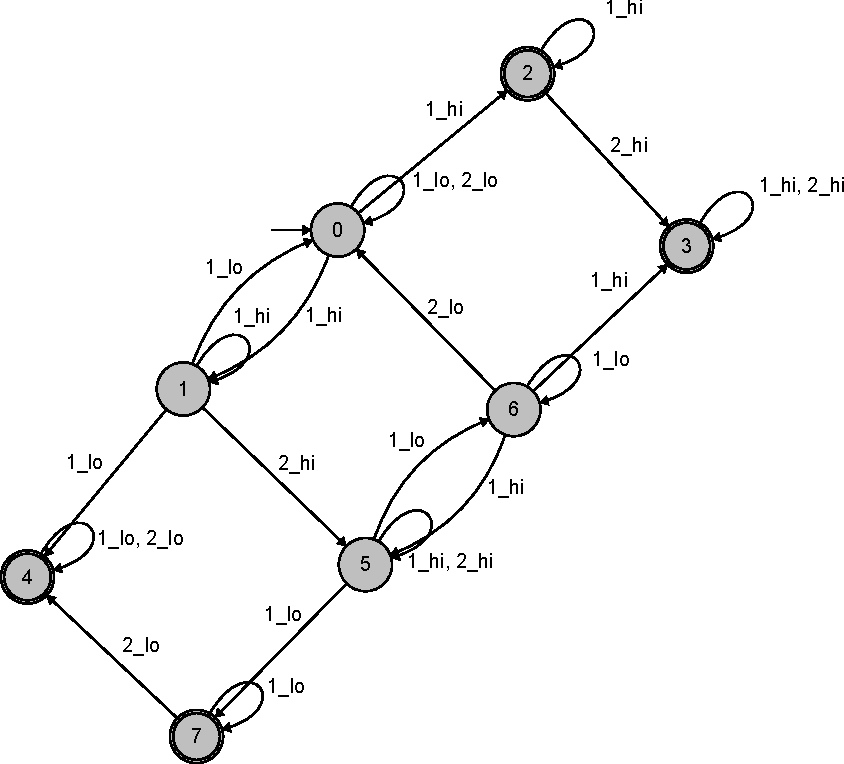
\includegraphics[scale=0.7]{lib_2do_fail2.pdf}
	\caption{The cause-effect fault automaton model (left), and the resulting
	composition of two components (right)}
	\label{fig:lib_2do_fail2}
\end{figure}

\begin{figure}[!th]
	\centering
	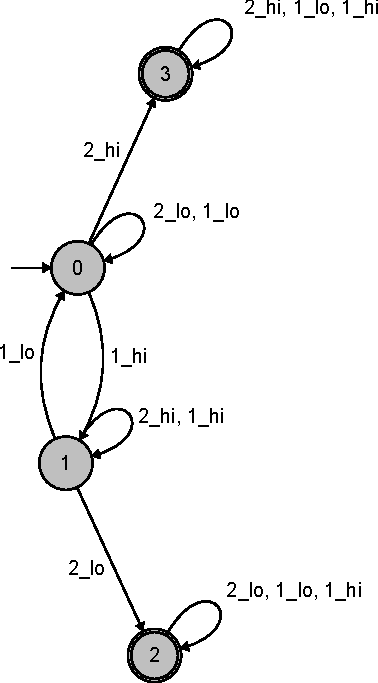
\includegraphics[scale=0.7]{lib_do2do_fail3.pdf}
	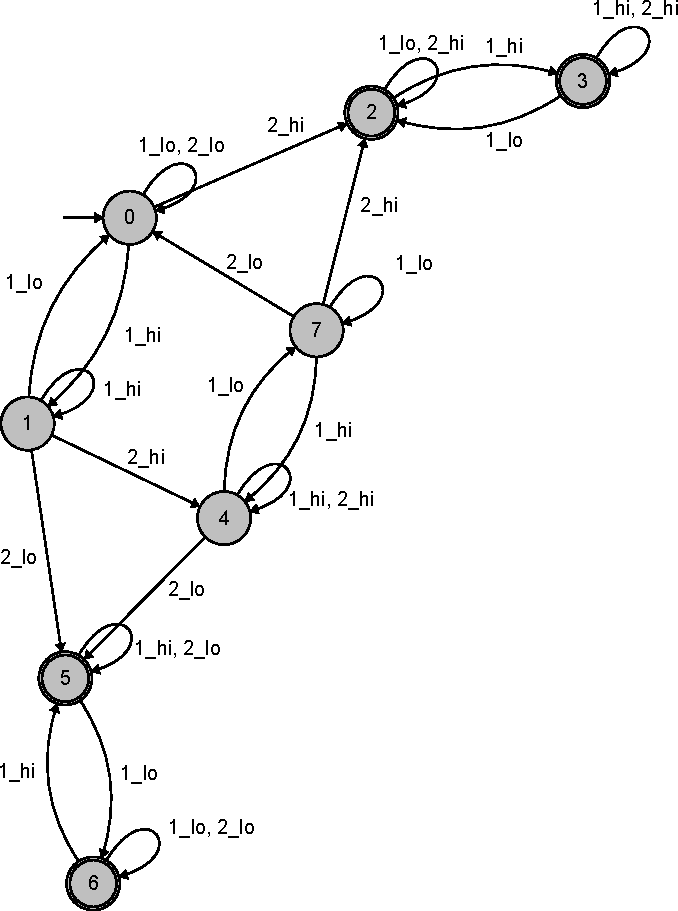
\includegraphics[scale=0.7]{lib_2do_fail3.pdf}
	\caption{The model of the constrain (left) and the composition result (right).
	Failures are in the second (i.e. ``effect") module}
	\label{fig:lib_2do_fail3}
\end{figure}

A consequent connection of two modules: $1$ -- ``cause'' (e.g. a contactor) and
$2$ -- ``effect'' (e.g. a motor), where the second module has failures is
depicted in Figure \ref{fig:lib_2do_fail3}. Here the failures are modeled using
state-based failure approach.


\section{Valve}

The most known physical model of a valve is depicted in the Figure
\ref{fig:lib_valve}.
The model reflects a wide variety of valves, e.g. gate valves, butterfly valves,
ball valves, etc. In general, five states if this type of equipment can be
distinguished: two boundary states (closed and open), two movement states
(opening, closing) and stop in an intermediate position.

The ``stop'' position of the gate valve model can be marked as faulty,
since gate valves must usually stay either closed or open.

\begin{figure}[!th]
	\centering
	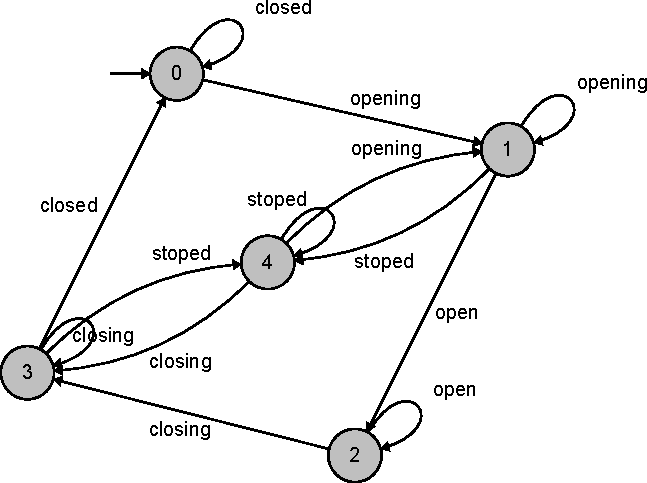
\includegraphics[scale=0.7]{lib_valve.pdf}
	\caption{Automaton model of a valve}
	\label{fig:lib_valve}
\end{figure}


\subsection{Valve with sensors}

Figure \ref{fig:lib_valve2sensor1} shows the model of a sensor $1$ built
according to the model of two-state components described before, and a constrain
model which assumes that the sensor observes ``closed'' state of the valve.
From the perspective of the sensor the valve can be either closed or not. In
another words, the valve is seen as a two-state component. Thus, the constrain
automaton similar to the one shown in the Figure \ref{fig:lib_2do} can be used.

\begin{figure}[th]
	\centering
	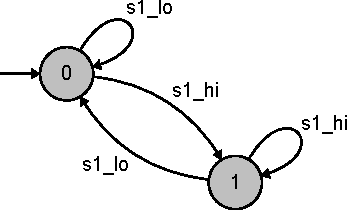
\includegraphics[scale=0.7]{lib_sensor1.pdf}
	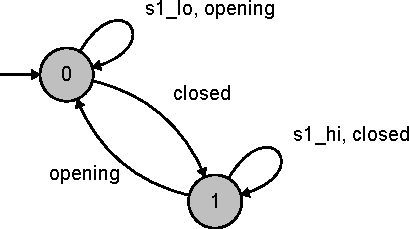
\includegraphics[scale=0.7]{lib_valve2sensor1.pdf}	
	\caption{Automata of a sensor and a constrain model for the sensor--valve
	relationship}
	\label{fig:lib_valve2sensor1}
\end{figure}

Let the valve to have two sensor: one for the closed state and another
one for the open state. An inference diagram of such system is shown in the
Figure \ref{fig:lib_id_valve+2sensors}. It reflects the coupling of all the
corresponding models, e.g. valve, two sensors ($S1$, $S2$) and their
constrains. The result of the composition of is depicted in the Figure
\ref{fig:lib_valve+2sensors}. The purpose of the figure is to show the level of
complexity of such simple system.

A fault model of the valve's sensors is equal to the one depicted in the Figure
\ref{fig:lib_dido_fail}.

\begin{figure}[!th]
	\centering
	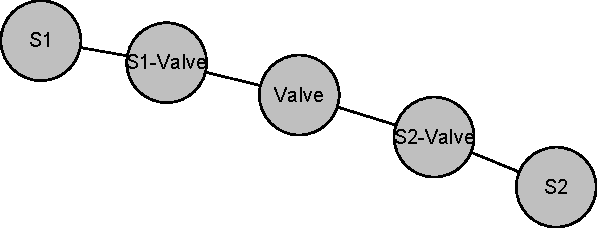
\includegraphics[scale=0.7]{lib_id_valve+2sensors.pdf}
	\caption{Inference diagram of a valve with two sensors}
	\label{fig:lib_id_valve+2sensors}
\end{figure}

 
\begin{figure}[th]
	\centering
	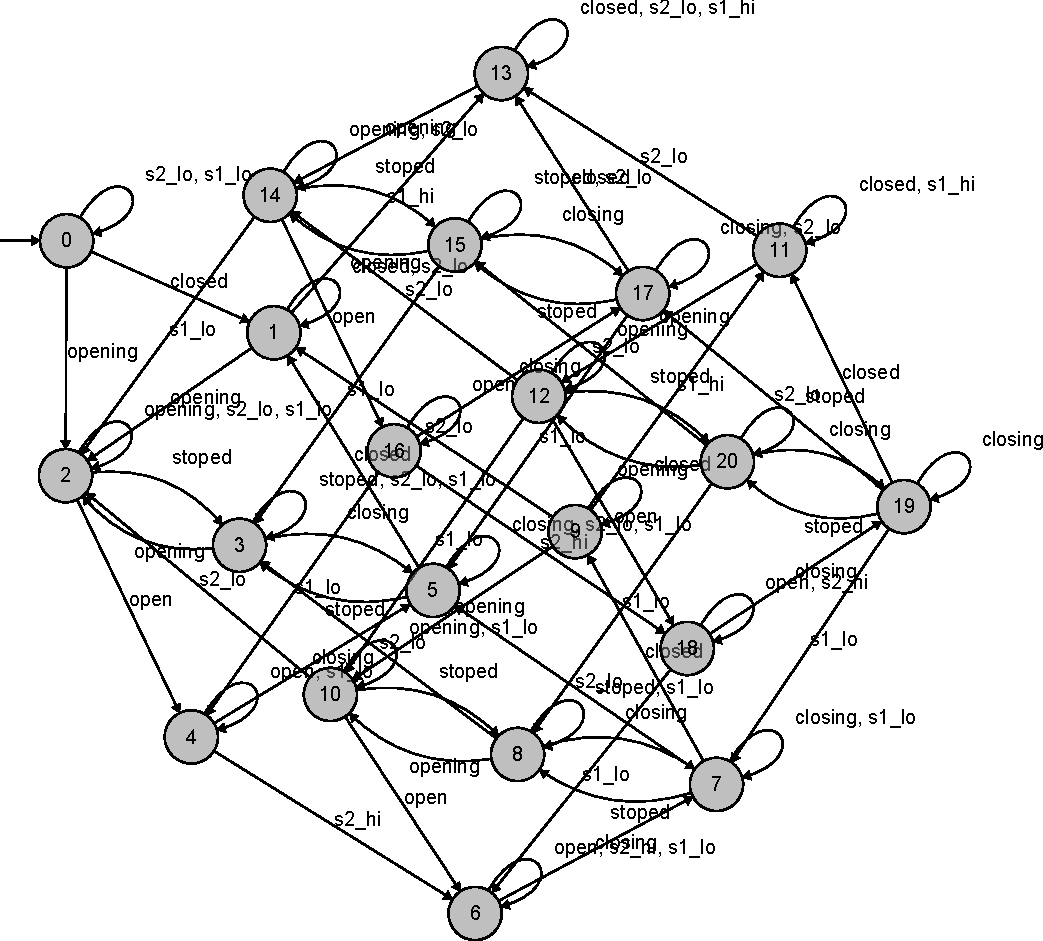
\includegraphics[scale=0.7]{lib_valve+2sensors.pdf}
	\caption{Automaton of a valve with two sensors (open and closed)}
	\label{fig:lib_valve+2sensors}
\end{figure}


\subsection{Valve with actuator} 

Automaton model of a double actuation device for a valve is depicted in the
Figure \ref{fig:lib_act} (think of an bidirectional motor). Actually, it has two
actuating parts, denoted in the figure by  prefixes $a$ and $b$. Part $a$ is responsible for the ``opening''
movement, part $b$ is responsible for the ``closing'' movement. Each actuating
part is equal to the two-state digital component model, presented before.
In the composition of these two components a consequent execution of events
$a_hi$ and $b_hi$ is forbidden, i.e. it is necessary that $a\_hi \Rightarrow
b\_lo$ and $b\_hi \Rightarrow a\_lo$.

\begin{figure}[!ht]
	\centering
	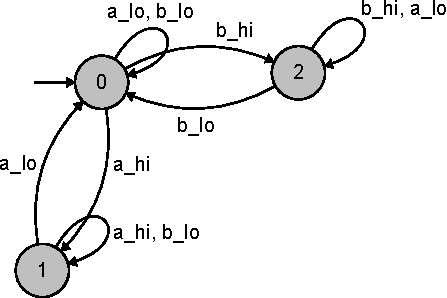
\includegraphics[scale=0.7]{lib_act.pdf}
	\caption{Automaton of a valve actuator}
	\label{fig:lib_act}
\end{figure}


\begin{figure}[!ht]
	\centering  
	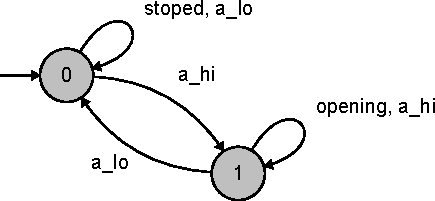
\includegraphics[scale=0.7]{lib_valve2actuator_a.pdf}
	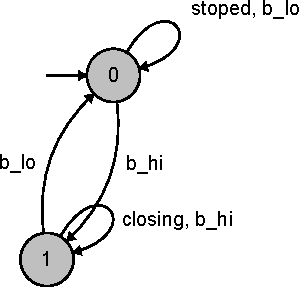
\includegraphics[scale=0.7]{lib_valve2actuator_b.pdf}
	\caption{Automata of the valve actuator constrains}
	\label{fig:lib_valve2actuator_a}
\end{figure}

The actuation devices are coupled with the physical valve model through a 
constrain automaton, similar to described above. The constrain automata for
the valve are shown in the Figure \ref{fig:lib_valve2actuator_a}. 
The result of the composition of the valve, actuator and constrains is depicted
in the Figure \ref{fig:lib_valve+actuator}. Marked states are correspond to the
``stop'' state of the valve, which may be considered as a fault for a
gate valve.

\begin{figure}[!ht]
	\centering
	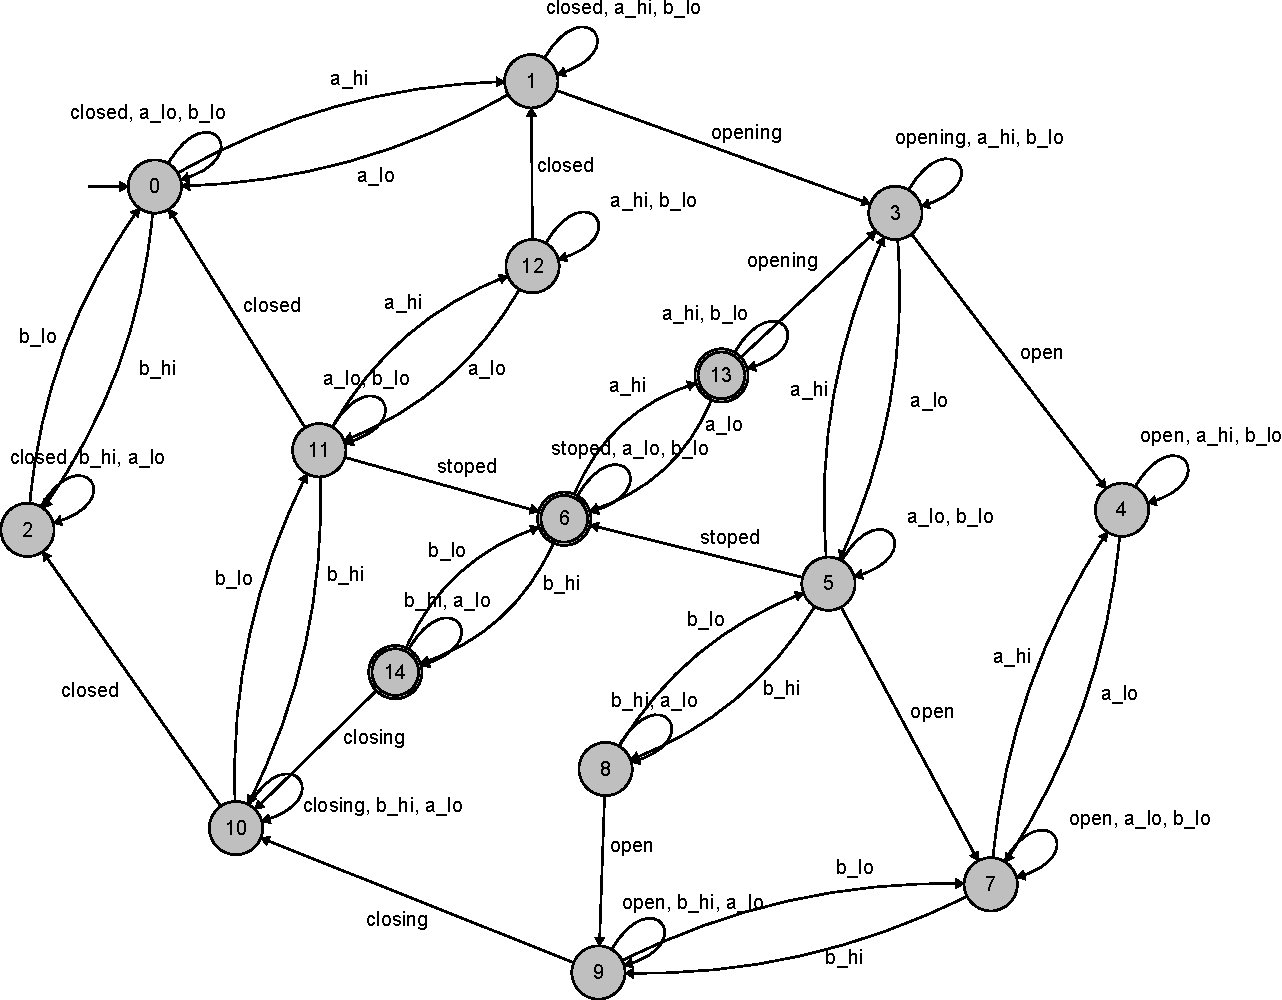
\includegraphics[scale=0.7]{lib_valve+actuator.pdf}
	\caption{Automaton of a valve with the actuator}
	\label{fig:lib_valve+actuator}
\end{figure}


\subsection{Valve with sensors and actuator}

Automaton which represents the complete model, i.e. the composition of the valve
with two sensors and the actuator has 63 states and 424 transitions. A
corresponding inference diagram is shown in the Figure
\ref{fig:lib_valve+2sensors+actuator}. Meaning of the nodes names is explained
in the table below.

\begin{figure}[!ht]
	\centering
	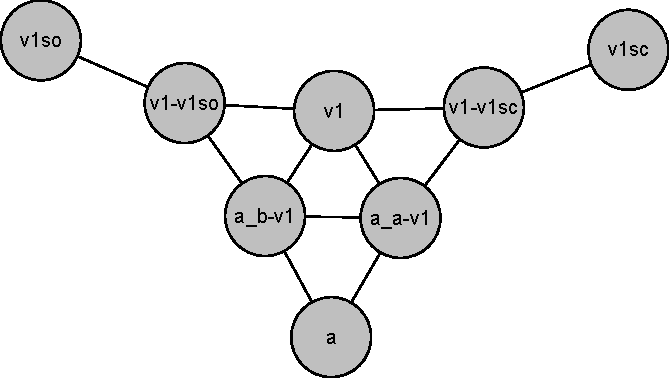
\includegraphics[scale=0.7]{lib_valve+2sensors+actuator.pdf}
	\caption{Inference diagram of a valve with two sensor and an actuator (see
	Table \ref{tbl:id_valve+2sensors+actuator} for the nodes names description)}
	\label{fig:lib_valve+2sensors+actuator}
\end{figure}

\begin{table}[!ht]
\caption{Nodes labels of the inference diagram of the valve, sensors and
actuator}
\centering
	\begin{tabular}{l l}
	\\	
	Node label & Description\\
	\hline
	v1 & Valve\\
	v1so & Sensor ``Open"\\
	v1sc & Sensor ``Closed"\\
	v1-v1so & Constrain of the valve to the sensor ``Open"\\
	v1-v1sc & Constrain of the valve to the sensor ``Closed"\\
	a & Actuator\\
	a\_a-v1 & Constrain of the valve to the actuator's part ``Opening"\\
	a\_b-v1 & Constrain of the valve to the actuator's part ``Closing"
	\end{tabular}
	\label{tbl:id_valve+2sensors+actuator}
\end{table}



\clearpage
\newpage
